\documentclass[compress,11pt]{beamer}
%\includeonly{pendel}
\usetheme{Ilmenau}
%\usetheme{fau-4-3}
%\usecolortheme{beaver}
%\beamertemplatenavigationsymbolsempty
\usepackage[ngerman]{babel}
\usepackage{marvosym}
\usepackage{multimedia}
\usepackage[utf8]{inputenc}
\usepackage{amsmath}
\usepackage{amsfonts}
\usepackage{amssymb}
\usepackage{graphicx}
\usepackage{esvect}
%\author{}
\title{EP Gruppe 8}
%\setbeamercovered{transparent}
%\setbeamertemplate{navigation symbols}{}
%\logo{}
%\institute{}
%\date{}
%\subject{}
\usepackage{verbatim}
\begin{document}


\section{Aufgabe 1: Komponenten eines Lock-In-Verstärkers}
\subsection{Grobe Funktionsweise eines Lock-In Verstärkers}
\begin{frame}
\begin{block}
\begin{itemize}
\item Lock-In Verstärker verstärken schwache Signale, die mit einer bekannten Frequenz modulieren
\item Eingangssignal (schwach oder von Rauschen überlagert) wird mit Referenzsignal gleicher Frequent multipliziert
\item Falls Signal Rechteck-förmig (wird im folgenden realisiert), kann die Multiplikation der Signale durch Analogschalter bewerkstelligt werden
\end{itemize}
\end{block}
Im folgenden werden die einzelnen Komponenten eines Lock-In Verstärkers zusammengebaut und getestet
\end{frame}
\subsection{Phasenschieber}

\begin{frame}
Aufzubauen war folgende Schaltung:\\
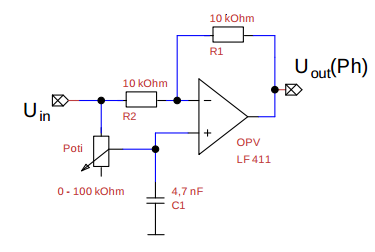
\includegraphics[width=.7\textwidth]{schalt/phasenschieber}\\

\end{frame}
\begin{frame}
\begin{block}{Funktionsweise der Schaltung}
\begin{itemize}
\item Op-Amp verstärkt mit $|V| = 1$
\item Poti und Kondensator wirken als Tiefpass, der die Phase verschiebt
\end{itemize}
\end{block}
Phasenschieber und alle weiteren Bautelie Lock-Ins wurden mit einem sinusförmigen Teststrom von $U_{pp} = 1 V$ und $f = 777 Hz$ betrieben
\end{frame}
\begin{frame}
Es wurden mittels Potentiometer verschiedene Phasen eingestellt und die dazugehörigen Potentiometerwiderstände gemessen:\\
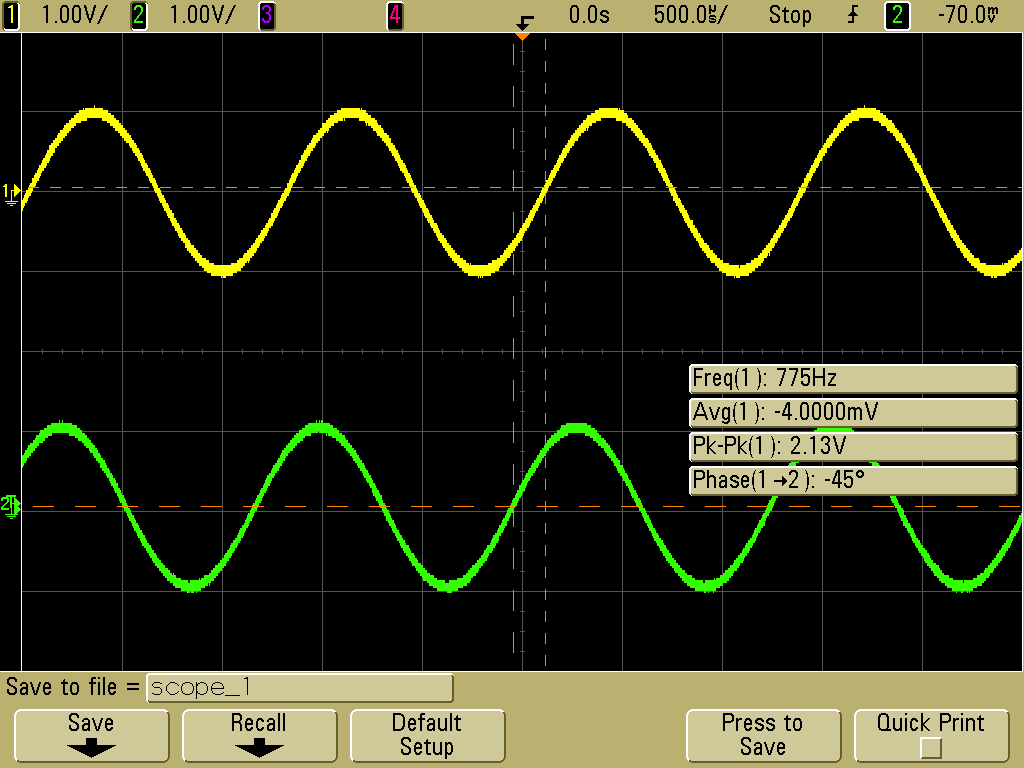
\includegraphics[width=.7\textwidth]{../oszi/scope_1}\\
Beispiel für das sich ergebende Bild am Oszilloskop

\end{frame}
\begin{frame}
\begin{tabular}{|c|c|}
\hline
Phase & zugehöriger $R_{Pot}$ in $k \Omega$  \\
\hline
    -176 & 0.0015 ($R_{Pot,min}$) \\
    45 & 18.1 \\
    91 & 43.9 \\
	120 & 78.94 \\
	
	
\hline
\end{tabular}

\end{frame}
\begin{frame}
Herleitung der Theoriekurve zur Phasenverschiebung:\\
Es ergibt sich für die Spannungen an den Eingängen:
\begin{equation}
U_{+} = U_{in} \cdot \frac{Z_{C_1}}{Z_{C_1} + R_{pot}}
\end{equation}
\begin{equation}
U_{-} = U_{in} \frac{R_2}{R_1 + R_2} \cdot (U_{out} - U_{in})
\end{equation}
Benutze nun goldene Regel:
\begin{equation}
\Rightarrow U_{out} = U_{in} \cdot \frac{Z_{C1} - R_{pot}}{Z_{C} + R_{pot}}
\end{equation}
Nach Betragsetzung $|U_{out}| = |U_{in}|$ ergibt sich:
\begin{equation}
\phi = \arctan (\frac{4 \cdot \pi \cdot f \cdot R_{pot} \cdot C }{1 - (2 \cdot \pi \cdot f \cdot R_{pot} \cdot C)^2})
\end{equation}
\end{frame}
\begin{frame}
plot kaputt (hab vermutlich einen fehler im plotskript und den nicht mehr gefunden)\\
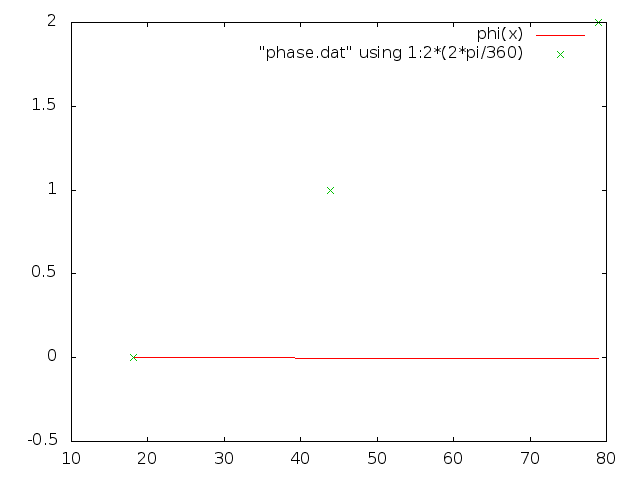
\includegraphics[width=.7\textwidth]{../phase}
\end{frame}



\subsection{Komparatoren}
\begin{frame}
Schaltplan:\\
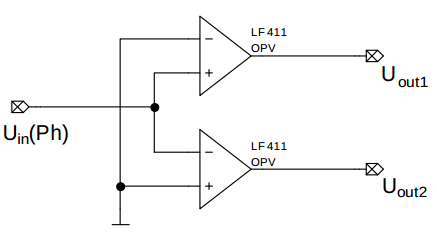
\includegraphics[width=.7\textwidth]{schalt/komparator}
\end{frame}
\begin{frame}
\begin{block}{Funktionsweise der Schaltung}
\begin{itemize}
\item Operationsverstärker ohne Gegenkopplung funktioniert als Komparator
\item ideales Bauteil gibt bei $U_{versorgung} = \pm 7 V$ ein $U_{out} = sign(U_3 - U_2) \cdot U_{versorgung}$ aus
\item Pin 2 bzw. Pin 3 werden geerdet, $U_{in}$ liegt jeweils am anderen Pin an $\Rightarrow$ Ein Op-Amp. invertiert, der andere nicht
\end{itemize}
\end{block}
Schaltung gibt zwei zueinander inverse, sonst identische Rechtecksspannungen aus\\
Verstärkung gleich 1, 
\end{frame}
\begin{frame}
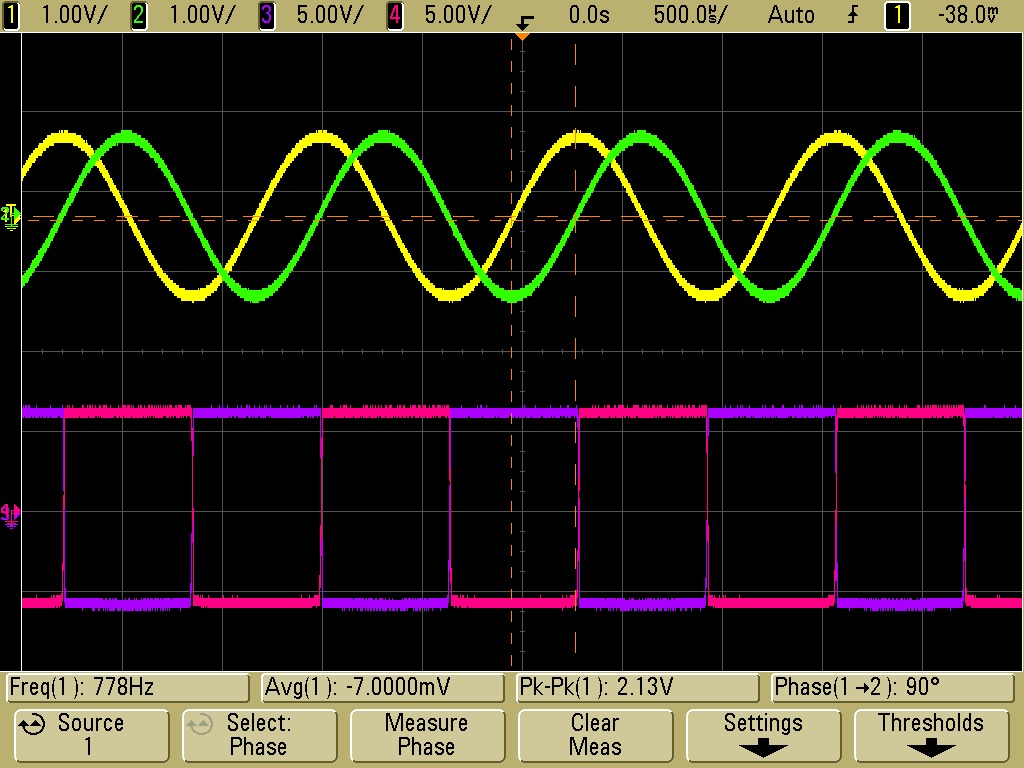
\includegraphics[width=.7\textwidth]{../oszi/scope_5}\\
Vergleich der von $U_{generator}$, $U_{in}$, $U_{out,1}$ und $U_{out,2}$
\end{frame}




\subsection{Eingangsverstärker}
\begin{frame}
Schaltung:\\
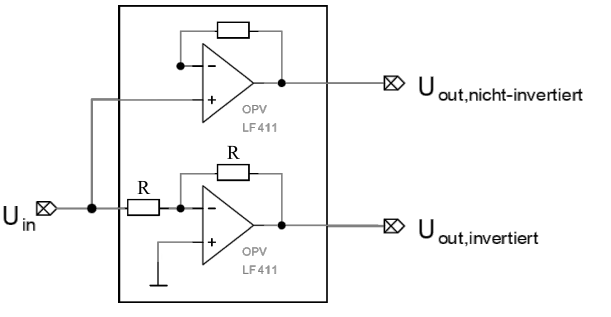
\includegraphics[width=.7\textwidth]{schalt/eingangs}\\
Beide Schaltungen verstärken mit Faktor 1, obere normal (da $U_{in}$ auf Pin 3 trifft), untere invertiert (da $U_{in}$ auf invertierenden Pin 2 trifft)
\end{frame}
\begin{frame}
Es ergibt sich am Oszilloskop folgendes Bild:\\
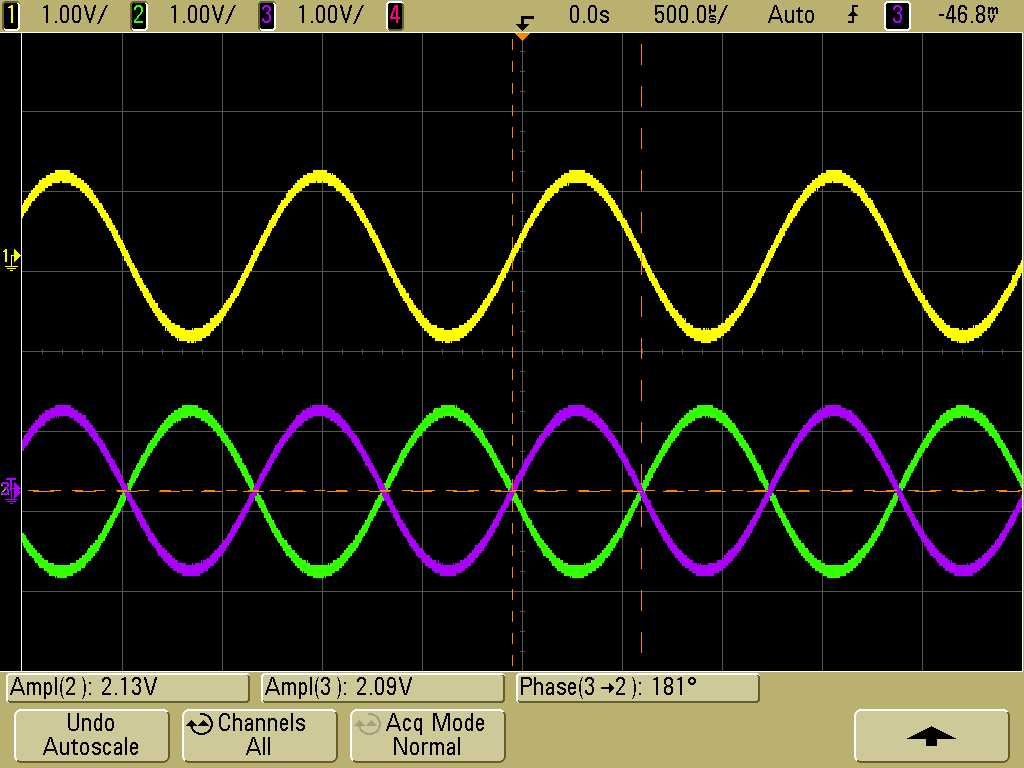
\includegraphics[width=.7\textwidth]{../oszi/scope_8}
\end{frame}

\subsection{Analogschalter}
\begin{frame}
Bisherige Schaltungen (Phasenverschieber, Komperatoren, Verstärker) werden nun miteinander zum Lock-In-Verstärker zusammengefügt:\\
%Schaltung
Benötogtes Bauteil ist ein Analogschalter
\end{frame}
\subsubsection{Einschub: Analogschalter}
\begin{frame}
Schaltplan des Bauteils:\\
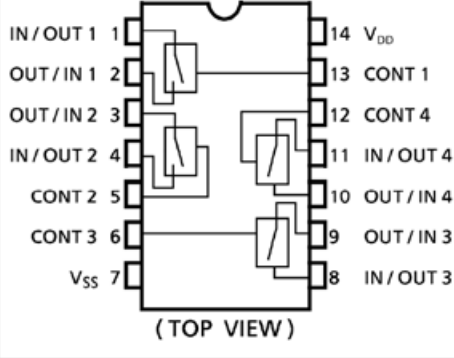
\includegraphics[width=.7\textwidth]{schalt/analog}
\end{frame}
\begin{frame}
\begin{block}{Funktionsweise eines Analogschalters}
\begin{itemize}
\item Technische Realisierung des Schalters durch Feldeffekt-Transistoren
\item Schalter schließt ($R \approx 10^6 \Omega$), wenn Potential des zugehörigen "Control"-Pins gleich $V_{DD}$ ist
\item Schalter ist offen, wenn Pin-Potential gleich $V_{SS}$
\end{itemize}
\end{block}
\end{frame}
\begin{frame}
Vervollständigt wird Schaltung noch mit Tiefpass:\\
Grenzfrequenz:
\begin{equation}
f = \frac{1}{2 \cdot \pi \cdot F \cdot R} \approx 1.59 Hz
\end{equation}
\begin{block}{Fazit}
Alle Komponenten des Lock-In-Verstärkers funktionieren wie erwartet
\end{block}
\end{frame}

\end{document}
